In this section, we will be a taking look at the necessary definitions and theoretical fundamentals of various technical terms introduced in this report. 
This will help us understand the fundamentals of all the concepts used throughout the thesis. We will take a look at the following concepts; 
SceneFun3D tasks and their importance, 3D scene graphs and their uses, methods for generating scene graphs, semantic and instance segmentation of objects, 
approaches for achieving semantic and instance segmentation, the foundation models used and their rationale, and finally, open-vocabulary object detection.
The section will include figures and examples as they are easier to comprehend as compared to text for complex concepts. Although the content of this 
chapter is thorough it is just a brief description of the actual concepts limited to the necessity of this thesis.

\section{SceneFun3D tasks}
The authors of \cite{delitzas2024scenefun3d} introduce three challenging tasks in their paper. We tackle the first two tasks to achieve the 
objectives defined in our thesis. The three tasks are:
\begin{compactenum}[1.]
\item	Functionality segmentation.
\item	Task-driven affordance grounding.
\item	Motion estimation.
\end{compactenum}
The paper exerts pressure on the fact that these tasks are challenging even with today's advancements in 3D scene understanding
and 3D semantic and instance segmentation. Solving the task mentioned above will ensure that the system is capable of 
performing intricate tasks which require manipulating fine-grained functional elements of various objects.
For example, opening a door by turning the door handle. If we breakdown this simple task of opening a door into three parts
and then try to map them to the tasks mentioned above we get, task 1 functionality segmentation resembles segmenting out the door handle 
from the door frame, task 2 task-driven affordance grounding resembles the association of the text query to the actual 
instance of the door handle which can be turned. And finally, with motion estimation, we get the motion parameters such as direction, action and angle 
at which the handle needs to be turned. Thus, solving the three tasks effectively ensures that the system will be good at performing daily
tasks as delicately as a human. \\
\begin{figure}[ht!]
    \centering
    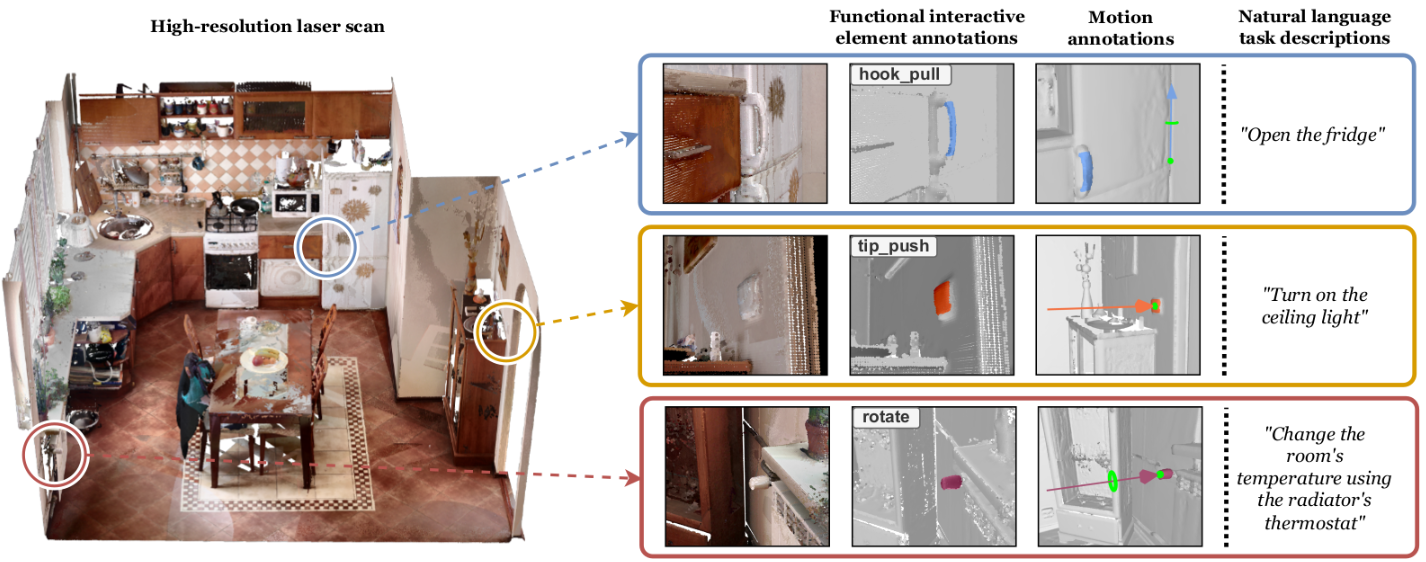
\includegraphics[width=\textwidth]{content/images/SceneFun3D.png}
    \caption{SceneFun3D tasks visualised \cite{delitzas2024scenefun3d}}
    \label{fig:your_image_label}
\end{figure}
\cref{fig:your_image_label} shows the expected output of all the three tasks. Functionality segmentation refers to segmenting out the functional interactive 
element from the given scene and annotating it with one of the eight affordance labels defined by \cite{gibson}. Task-driven affordance grounding refers to the task
of associating a text query in the context of the scene to the functional element that can be manipulated for the given text description. Finally, motion estimation
aims to provide the motion parameters that the agent should perform in order to successfully interact with the functional element.

Further, SceneFun3D also provides a well-defined dataset of 720 recorded scene from the ARKitScenes dataset and various assets for each scene 
to train deep learning models that can tackle these problems. They provide the following assets, RGB-D images, poses, accurate laser scans, 
annotations for each element present in the dataset, motion parameters for each annotation and task description in natural language for every function element.
In our thesis, we aim to beat the baseline results obtained by \citet{delitzas2024scenefun3d} for the first two tasks, namely 
functionality segmentation and task-driven affordance grounding. 

\section{3D scene graphs}
The term scene graph was first introduced in \cite{7298990}, as a novel framework for retrieval of images. Here, the authors designed the scene graph which 
consists of three sub-parts, the nodes, the edges and the attributes for each node. First, let us understand the definition of a scene graph and later
look at its evolution to 3D. \\
A scene graph can be defined as a structural representation of a particular scene which captures semantically rich information about the objects in that scene \cite{zhu2022scenegraphgenerationcomprehensive}.
This is done by explicitly modelling the objects, their attributes and the relationship between paired objects as seen in \cref{fig:2dvs3dSG}. The objects appear to be in boxes as nodes
and the spatial relationships are given by edges connecting the nodes.
In short, it is called a “scene graph” because it organizes all this information as a graph: the objects are represented as nodes with their attributes, and the edges between these 
nodes are the relationship between these objects. 

For a robot to navigate around its environment and interact with the objects in its vicinity, it first needs to have a semantically rich map of its surroundings. 
This surrounding area where the robot can move and interact is called the scene and the semantically rich map must contain the 
semantic data of all the objects in the scene as well as their locations and inter-object relationships. 
A 3D scene graph can be used to store this kind of semantically rich data of the objects of the robot’s surroundings. 

A 3D scene graph is an extension of the traditional scene graph. It is a spatial representation of the objects, their attributes 
and their relationships in three dimensions, in short, they store 3D information. The objects in 3D scene graphs are modelled as
 3D point clouds and they visually resemble the original object. The distinction between a normal scene graph and a 3d scene graph 
 can be seen from the \cref{fig:2dvs3dSG}
 \begin{figure}[ht!]
    \centering
    \includegraphics[width=\textwidth]{content/images/2dvs3dSG.png}
    \caption{3D (bottom left) vs 2D (bottom right) scene graph for given scene of two arm chairs (top)}
    \label{fig:2dvs3dSG}
\end{figure}
To further elaborate on 3D scene graphs, consider the example of a scene where an armchair is next to another armchair.
The scene graph here consists of two nodes;
the first node is the armchair with \enquote{red} as an attribute, and the second node is the second armchair with \enquote{red} as an attribute. The spatial relation, 
\enquote{next to} is given an edge. Thus, the scene graph provides a compact representation of the scene to the robot. 
An example can be seen from our implementation in the \cref{fig:2dvs3dSG}.

\subsection{Uses of 3D Scene Graph}
As we discussed above the scene graph can be leveraged by a robot to navigate around a scene and complete its tasks by manipulating objects defined in the task. 
Apart from this, there are numerous other tasks which can be accomplished using either a traditional scene graph or a 3D version of it. Scene graphs have been 
used to enhance image generation \cite{tripathi2019usingscenegraphcontext}, \cite{johnson2018imagegenerationscenegraphs}, 
the relationships between the nodes are leveraged to incorporate meaningful information during the image generation process to get realistic images.
 Other uses include image captioning using scene graphs \cite{8953305}. 
 Scene graphs can also be used to detect visual relationships between objects in an image, Visual question answering, semantic image retrieval and many more. \\
Before moving to the generation of 3D scene graphs, we will look at the tools used during this process. 
These tools are mainly machine learning and deep learning models. Scene graphs are generated from RGB-D images and poses. 
Out of these, RGB images play an important role in providing semantic information to the scene graph. RGB images are used for object detection,
object segmentation, relationship building and caption generation. All of these tasks are possible due to one or more foundation models.
Mainly foundation models like Visual Language Models such as LLaVA \cite{liu2023visualinstructiontuning} and GPT-4 \cite{openai2024gpt4technicalreport} are used for caption generation and 
relationship building, and SAM \cite{kirillov2023segment} for object segmentation. Along with this, object detection models like YOLO \cite{cheng2024yolow} form the basis of 
3D scene graph generation. 
Next, let us look at the theoretical concepts behind these models and then have a look at how they help in scene graph generation.
\section{Foundation models}
Foundation models can be defined as large-scale, pre-trained models that can perform various downstream tasks \cite{bommasani2022opportunitiesrisksfoundationmodels}. 
Foundation models have two reasons for being successful, scale and transfer learning. On one hand, Scale represents,
more computing power in terms of CPU, GPU and memory and a large amount of multimodal training data. Such data is gathered from 
massive datasets generated across diverse domains, this makes generalization possible in foundation models. On the other hand, transfer
learning takes the learnings from one task (e.g., object recognition in images) and
applies them to another task (e.g., activity recognition in videos). 
\begin{figure}[ht!]
    \centering
    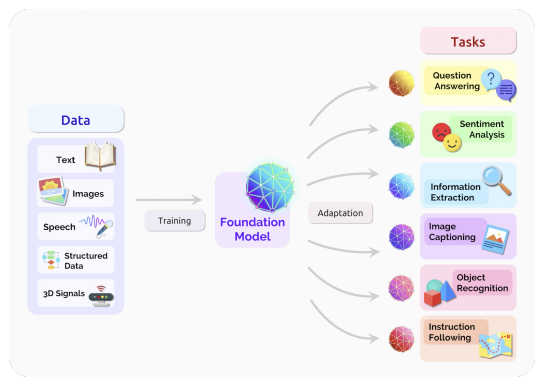
\includegraphics[width=\textwidth]{images/FoundationModels.png}
    \caption{Foundation model overview.}
    \label{fig:foundation_model}
\end{figure}
From \cref{fig:foundation_model} we can see that, 
a foundation model gathers the knowledge from all the data from various data sources such as texts, images, videos and many more.
This model then adapts to a wide range of downstream tasks such as question answering, sentiment analysis, and object detection just to 
name a few. Their applications range from natural language processing (NLP), and computer vision (CV) to robotics and more. 
Let us look at some of the foundation models we will be using in our scene graph implementation.

\subsection{Segment Anything Model}
The paper by \citet{kirillov2023segment} first introduced the Segment Anything Model (SAM). SAM is developed by Meta FAIR. 
This foundation model can segment any given 2D image. Segmentation can be made using the following ways, 
it can be prompted with interactive points and boxes, it can automatically segment everything in the image without a prompt, 
and generate multiple masks for ambiguous prompts. According to Meta AI, “Sam has learned a general notion of what objects are – this understanding enables zero-shot generalization to 
unfamiliar objects and images without requiring additional training.”. The outstanding accomplishments of SAM are possible due to the fact that
the authors used a large number of masks approximately 1 billion masks from 11 million images to train the model. Due to such a large dataset, 
the model has learnt to segment almost anything out of a given image, hence the name Segment Anything Model. In the figure below we can see the segmentation results from SAM.
A glimpse of SAM can be seen in the \cref{fig:sam}
\begin{figure}[ht!]
    \centering
    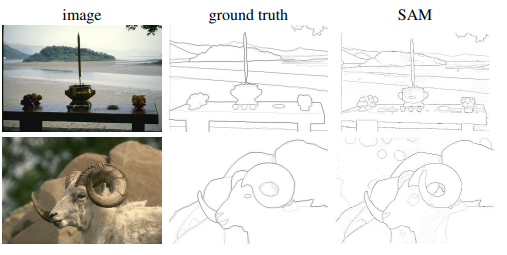
\includegraphics[width=\textwidth]{content/images/SAM.png}
    \caption{Foundation model overview. \cite{kirillov2023segment}}
    \label{fig:sam}
\end{figure}
\subsection{Vision Language Models}
Vision Language Models (VLMs) are advanced machine learning models able to process visual and textual data. VLMs are also foundation models as they are trained on multimodal data such as text, images,
videos and many more. Moreover, the ability of VLMs to generalize and provide answers to any given task may it be question answering, object detection or sentiment analysis makes
them worthy of foundation models. They can generate outputs based on their understanding of the multimodal input provided to them. 
In this chapter, we will be looking at the two most used VLMs, GPT-4 and LLaVA.

\subsubsection{GPT-4:}
The onset of the Large Language Model (LLM) in today's world has opened many possibilities for the use of AI. One such use is chatbot applications or AI
assistants. ChatGPT is a foundation model developed by OpenAI. ChatGPT was made public in November 2022. Initially, ChatGPT was only capable of 
text-based queries but performed well in question-answering tasks. It showed human-like rationale. However, it had limitations such as 
only a single mode of input and output (text) and it was poor in mathematical reasoning. Since then ChatGPT has evolved and today the successor 
GPT4 has not only overcome previous limitations but also improved logical and rational reasoning \cite{openai2024gpt4technicalreport}. GPT-4 showed more than 20\% increase in overall accuracy
on the  United States Medical Licensing Examination (USMLE) sample test and AMBOSS questions \url{https://www.amboss.com/us} \cite{Penny2024-qx}. Moreover, GPT-4 
also has multimodal input and output capabilities, making it suitable for visual question-ansewering. Visual question-answering is the task where
the model is given an image or a video and is asked questions related to the data provided. The questions are for example, 'Describe the scene given in 
the image.', 'What color is the table in the given image' or 'Is there a chair present in the scene? What is its spatial relationship with the table?'

\subsubsection{Large Language and Vision Assistant:}
 Large Language and Vision Assistant (LLaVA) is an end-to-end large multimodal model trained on data generated with the help of GPT-4 \cite{liu2023visualinstructiontuning}. 
 It connects the vision encoder and LLM for general-purpose visual and language queries. LLaVA performs well on vision queries. 
 Vision queries are queries where the model is provided with an image and a general query is asked regarding the image. 
 For eg, An image with a room is provided and the query can be, ”Is there a computer present in this image?”. LLaVA is an open-source model which is available on
 hugging face. It is a cost-effective alternative to ChatGPT with great performance but not at par with ChatGPT. LLaVA provides an API format with which queries can be made
 to the model by downloading it locally. The API expects an image and a prompt in the query. In the code snippet given in \cref{lst:lavaTheory}, we instantiate the model and its processor. We
 query LLaVA using an image of two red armchairs in a room and ask the following query, \enquote{Please describe the given image.} \cref{fig:llava} shows the image
 and the output.  


\begin{figure}[ht!]
    \centering
    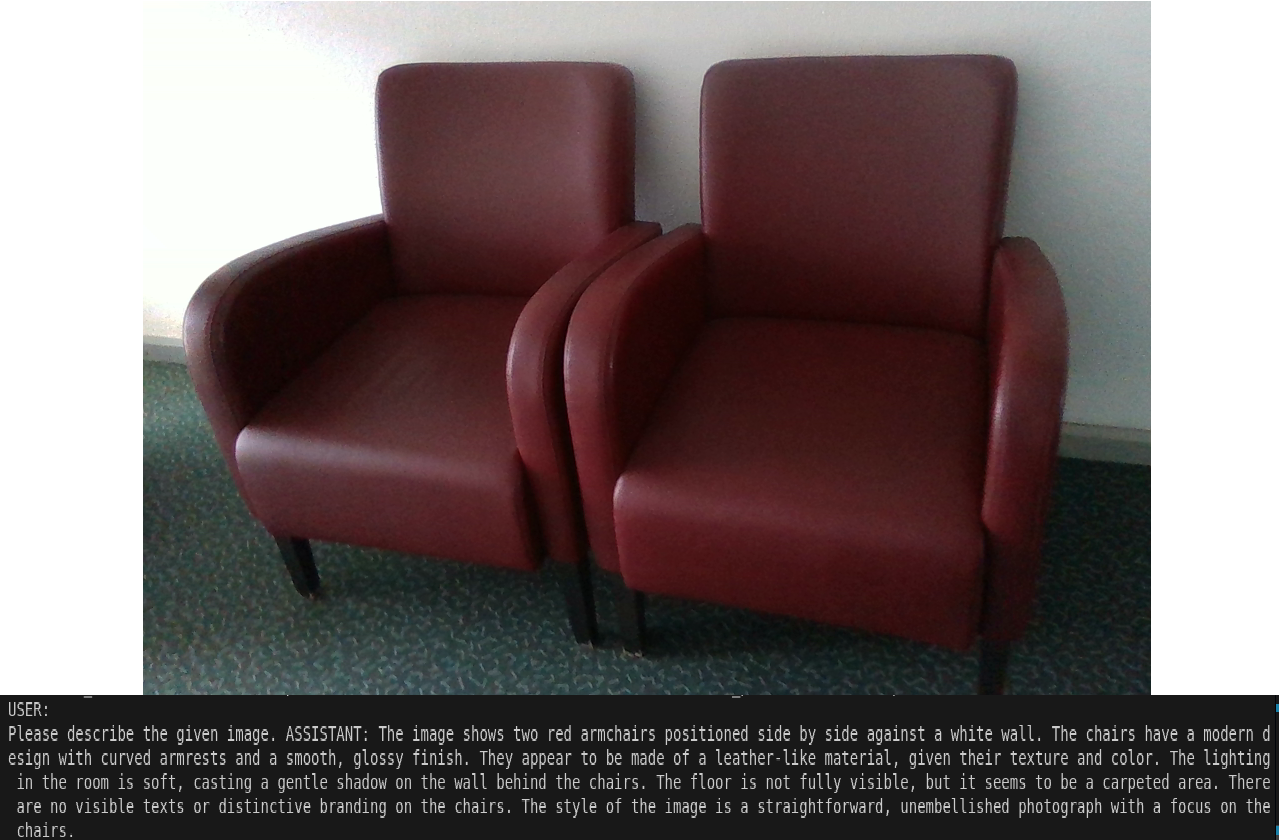
\includegraphics[width=\textwidth]{content/images/theory/LLaVA.png}
    \caption{Sample query on given image \cite{cheng2024yolow}}
    \label{fig:llava}
\end{figure}
 LLaVA can perform more complex tasks such as scene understanding or identifying spatial relationships, the example for this is given in \cref{chap:k7}.

\section{Object segmentation}
The task of separating an object from its background and other surrounding objects is called object segmentation. Object segmentation divides an image or 3D point cloud
 into meaningful regions, it labels each pixel or point to delineate the boundaries of different objects in the given scene. There are traditional methods like edge detection, 
 thresholding, and region growing which can segment out images. However, these methods do not provide good results in terms of semantic segmentation, where the segments must 
 have semantic information as a whole. For example, segmenting out a chair from a room. This is because traditional methods purely rely on 
 pixel-level features such as intensity, gradients, or texture, without understanding the context of objects present in the scene. However, newer methods like convolutional
 neural networks such as Mask R-CNN \cite{he2018maskrcnn}, transformer-based methods like SAM and point cloud networks like PointNet ++ are capable of semantic segmentation. 
 There are two types of object segmentation:
 \begin{compactenum}[1.]
    \item	Semantic segmentation.
    \item	Instance segmentation.
 \end{compactenum}
\begin{figure}[ht!]
    \centering
    \includegraphics[width=\textwidth]{content/images/segmentation_sem_vs_inst.png}
    \caption{Input image (top left), Semantic segmentation (top right), Instance segmentation (bottom right), Object detection (bottom left)}
    \label{fig:segmentation_sem_vs_inst}
\end{figure}
The difference between the two is that the former segments out object classes but doesn't consider objects under the same class as distinct segments whereas, the instance segment 
considers each segment as unique and identifies the obejcts in each class and consider them as a separate instances within the class. The difference can be understood by looking at 
\cref{fig:segmentation_sem_vs_inst} \cite{Sharma2022}. If we look at the top right part of the figure we see that there are two distinct colors yellow and red representing two
classes, nuts and bolts. Whereas, in the bottom right corner we can see each instance of the class nut has different colours and the same can be said for the class bolt.
\section{Open-vocabulary obejct detection}
The task of identifying an object and locating its position in an image is called object detection as seen in \cref{fig:segmentation_sem_vs_inst}. Until recently, object detection was limited to a small and fixed
set of classes. This limitation was due to the fact that obtaining a large training dataset with diverse classes is time-consuming and costly \cite{10.1007/978-3-031-20080-9_42}. 
The limitations of traditional object detection can be overcome using open-vocabulary object detection, a method where the model can detect the class of an 
object beyond its training set. Open-vocabulary object detection is a powerful method enabled by the advancements in powerful language encoders 
and contrastive image text training models like CLIP. 

One such model is YOLO-World by \citet{cheng2024yolow}, an approach to enhancing open vocabulary object detection capabilities in You Only Look Once (YOLO).
YOLO is a series of object detection models which are light-weight and effective. 
\begin{figure}[ht!]
    \centering
    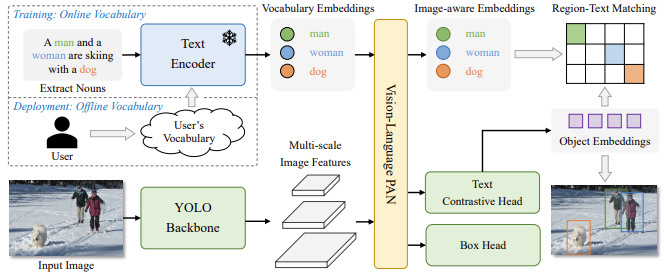
\includegraphics[width=\textwidth]{content/images/YOLOWorld.png}
    \caption{High-level working of YOLO-World \cite{cheng2024yolow}}
    \label{fig:yolo}
\end{figure}

The architecture of YOLO-World is given in \cref{fig:yolo}, it consists of a YOLOv8 detector, a Text encoder, and a Re-parameterizable Vision-Language
Path Aggregation Network (RepVL-PAN) \cite{cheng2024yolow}. Along with image the YOLO-World model also adopts text as input. The Text encoder is adopted
from a CLIP pretrained Transformer text encoder and it encodes the input text into text embeddings. The image is transformed into multi-scale image features using the 
YOLO backbone. The RepVL-PAN then enhances both text and image representation by fusing the image features and text embeddings. Finally, bounding boxes and object 
embeddings for matching the classes that appear in the input are predicted.

Applications for open-vocabulary object detection (OOVD) range from robotics to healthcare. In robotics, scene understanding, warehouse automation and household
assistance can be enhanced, the robots can predict unseen objects and understand the scene semantically better thus enabling human-like behaviour. In fields like Autonomous 
driving and security, OOVD can assist in detecting anomalies where the traditional object detection models may fail. The anomalies can be pedestrians, debris and
 road signs in autonomous driving or unattended baggage and unfamiliar objects in security surveillance.

 Despite its impressive capabilities, OOVD has many limitations that hold back its widespread adoption and accuracy in the real world. Some of the key limitations 
 include:
 \begin{compactenum}[1.]
    \item Generalization and accuracy: OOVD models struggle with rare categories for objects that lack visual-textual data in the training of text encoders like
    CLIP. Lack of expertise in domain-specific applications, as the OOVD models are good at generalization. 
    \item OOVD models depend on textual descriptions, limiting their performance to the quality of the text encoders used. Another limitation is the 
     language barrier as most text encoders are tarined in the English language, thus limiting the OOVD to English text descriptions. 
 \end{compactenum}
\section{Generating scene graphs using foundation models}
The foundation models like LLaVA, SAM, and the object detection model YOLO are utilised to create 3D scene graphs from a 
sequence of RGB-D images and camera poses. The RGB-D images are iterated and passsed to an object detection model first. The 
detection model returns the bounding boxes and classes of the detected objects in the RGB image. Later, these bounding boxes 
are passed to a segmentation model. The model returns the mask for each object in the RGB image. Next, the depth values from D images are 
utilised along with the mask to generate a 3D point cloud for the object. Finally the camera pose is applied to map the 
3D point cloud to the scene graph cordinate system. After all the objects have been mapped, the RGB image is passed to a 
VLM in order to get the spatial relationships between the detected objects. These spatial relationships are encoded as 
edges. The actual implementation and code snippets are given in \cref{chap:k7} 
